\documentclass{article} % For LaTeX2e
\usepackage{iclr2021_conference,times}

% Optional math commands from https://github.com/goodfeli/dlbook_notation.
% DO NOT MODIFY THIS COMMENT
% read `https://github.com/James-Yu/LaTeX-Workshop/wiki/Compile#the-root-file`
% read `https://github.com/James-Yu/LaTeX-Workshop/issues/1165`
% !TEX root = iclr2021_conference.tex

%%%%% NEW MATH DEFINITIONS %%%%%

\usepackage{amsmath,amsfonts,bm}

% Mark sections of captions for referring to divisions of figures
\newcommand{\figleft}{{\em (Left)}}
\newcommand{\figcenter}{{\em (Center)}}
\newcommand{\figright}{{\em (Right)}}
\newcommand{\figtop}{{\em (Top)}}
\newcommand{\figbottom}{{\em (Bottom)}}
\newcommand{\captiona}{{\em (a)}}
\newcommand{\captionb}{{\em (b)}}
\newcommand{\captionc}{{\em (c)}}
\newcommand{\captiond}{{\em (d)}}

% Highlight a newly defined term
\newcommand{\newterm}[1]{{\bf #1}}


% Figure reference, lower-case.
\def\figref#1{figure~\ref{#1}}
% Figure reference, capital. For start of sentence
\def\Figref#1{Figure~\ref{#1}}
\def\twofigref#1#2{figures \ref{#1} and \ref{#2}}
\def\quadfigref#1#2#3#4{figures \ref{#1}, \ref{#2}, \ref{#3} and \ref{#4}}
% Section reference, lower-case.
\def\secref#1{section~\ref{#1}}
% Section reference, capital.
\def\Secref#1{Section~\ref{#1}}
% Reference to two sections.
\def\twosecrefs#1#2{sections \ref{#1} and \ref{#2}}
% Reference to three sections.
\def\secrefs#1#2#3{sections \ref{#1}, \ref{#2} and \ref{#3}}
% Reference to an equation, lower-case.
\def\eqref#1{equation~\ref{#1}}
% Reference to an equation, upper case
\def\Eqref#1{Equation~\ref{#1}}
% A raw reference to an equation---avoid using if possible
\def\plaineqref#1{\ref{#1}}
% Reference to a chapter, lower-case.
\def\chapref#1{chapter~\ref{#1}}
% Reference to an equation, upper case.
\def\Chapref#1{Chapter~\ref{#1}}
% Reference to a range of chapters
\def\rangechapref#1#2{chapters\ref{#1}--\ref{#2}}
% Reference to an algorithm, lower-case.
\def\algref#1{algorithm~\ref{#1}}
% Reference to an algorithm, upper case.
\def\Algref#1{Algorithm~\ref{#1}}
\def\twoalgref#1#2{algorithms \ref{#1} and \ref{#2}}
\def\Twoalgref#1#2{Algorithms \ref{#1} and \ref{#2}}
% Reference to a part, lower case
\def\partref#1{part~\ref{#1}}
% Reference to a part, upper case
\def\Partref#1{Part~\ref{#1}}
\def\twopartref#1#2{parts \ref{#1} and \ref{#2}}

\def\ceil#1{\lceil #1 \rceil}
\def\floor#1{\lfloor #1 \rfloor}
\def\1{\bm{1}}
\newcommand{\train}{\mathcal{D}}
\newcommand{\valid}{\mathcal{D_{\mathrm{valid}}}}
\newcommand{\test}{\mathcal{D_{\mathrm{test}}}}

\def\eps{{\epsilon}}


% Random variables
\def\reta{{\textnormal{$\eta$}}}
\def\ra{{\textnormal{a}}}
\def\rb{{\textnormal{b}}}
\def\rc{{\textnormal{c}}}
\def\rd{{\textnormal{d}}}
\def\re{{\textnormal{e}}}
\def\rf{{\textnormal{f}}}
\def\rg{{\textnormal{g}}}
\def\rh{{\textnormal{h}}}
\def\ri{{\textnormal{i}}}
\def\rj{{\textnormal{j}}}
\def\rk{{\textnormal{k}}}
\def\rl{{\textnormal{l}}}
% rm is already a command, just don't name any random variables m
\def\rn{{\textnormal{n}}}
\def\ro{{\textnormal{o}}}
\def\rp{{\textnormal{p}}}
\def\rq{{\textnormal{q}}}
\def\rr{{\textnormal{r}}}
\def\rs{{\textnormal{s}}}
\def\rt{{\textnormal{t}}}
\def\ru{{\textnormal{u}}}
\def\rv{{\textnormal{v}}}
\def\rw{{\textnormal{w}}}
\def\rx{{\textnormal{x}}}
\def\ry{{\textnormal{y}}}
\def\rz{{\textnormal{z}}}

% Random vectors
\def\rvepsilon{{\mathbf{\epsilon}}}
\def\rvtheta{{\mathbf{\theta}}}
\def\rva{{\mathbf{a}}}
\def\rvb{{\mathbf{b}}}
\def\rvc{{\mathbf{c}}}
\def\rvd{{\mathbf{d}}}
\def\rve{{\mathbf{e}}}
\def\rvf{{\mathbf{f}}}
\def\rvg{{\mathbf{g}}}
\def\rvh{{\mathbf{h}}}
\def\rvu{{\mathbf{i}}}
\def\rvj{{\mathbf{j}}}
\def\rvk{{\mathbf{k}}}
\def\rvl{{\mathbf{l}}}
\def\rvm{{\mathbf{m}}}
\def\rvn{{\mathbf{n}}}
\def\rvo{{\mathbf{o}}}
\def\rvp{{\mathbf{p}}}
\def\rvq{{\mathbf{q}}}
\def\rvr{{\mathbf{r}}}
\def\rvs{{\mathbf{s}}}
\def\rvt{{\mathbf{t}}}
\def\rvu{{\mathbf{u}}}
\def\rvv{{\mathbf{v}}}
\def\rvw{{\mathbf{w}}}
\def\rvx{{\mathbf{x}}}
\def\rvy{{\mathbf{y}}}
\def\rvz{{\mathbf{z}}}

% Elements of random vectors
\def\erva{{\textnormal{a}}}
\def\ervb{{\textnormal{b}}}
\def\ervc{{\textnormal{c}}}
\def\ervd{{\textnormal{d}}}
\def\erve{{\textnormal{e}}}
\def\ervf{{\textnormal{f}}}
\def\ervg{{\textnormal{g}}}
\def\ervh{{\textnormal{h}}}
\def\ervi{{\textnormal{i}}}
\def\ervj{{\textnormal{j}}}
\def\ervk{{\textnormal{k}}}
\def\ervl{{\textnormal{l}}}
\def\ervm{{\textnormal{m}}}
\def\ervn{{\textnormal{n}}}
\def\ervo{{\textnormal{o}}}
\def\ervp{{\textnormal{p}}}
\def\ervq{{\textnormal{q}}}
\def\ervr{{\textnormal{r}}}
\def\ervs{{\textnormal{s}}}
\def\ervt{{\textnormal{t}}}
\def\ervu{{\textnormal{u}}}
\def\ervv{{\textnormal{v}}}
\def\ervw{{\textnormal{w}}}
\def\ervx{{\textnormal{x}}}
\def\ervy{{\textnormal{y}}}
\def\ervz{{\textnormal{z}}}

% Random matrices
\def\rmA{{\mathbf{A}}}
\def\rmB{{\mathbf{B}}}
\def\rmC{{\mathbf{C}}}
\def\rmD{{\mathbf{D}}}
\def\rmE{{\mathbf{E}}}
\def\rmF{{\mathbf{F}}}
\def\rmG{{\mathbf{G}}}
\def\rmH{{\mathbf{H}}}
\def\rmI{{\mathbf{I}}}
\def\rmJ{{\mathbf{J}}}
\def\rmK{{\mathbf{K}}}
\def\rmL{{\mathbf{L}}}
\def\rmM{{\mathbf{M}}}
\def\rmN{{\mathbf{N}}}
\def\rmO{{\mathbf{O}}}
\def\rmP{{\mathbf{P}}}
\def\rmQ{{\mathbf{Q}}}
\def\rmR{{\mathbf{R}}}
\def\rmS{{\mathbf{S}}}
\def\rmT{{\mathbf{T}}}
\def\rmU{{\mathbf{U}}}
\def\rmV{{\mathbf{V}}}
\def\rmW{{\mathbf{W}}}
\def\rmX{{\mathbf{X}}}
\def\rmY{{\mathbf{Y}}}
\def\rmZ{{\mathbf{Z}}}

% Elements of random matrices
\def\ermA{{\textnormal{A}}}
\def\ermB{{\textnormal{B}}}
\def\ermC{{\textnormal{C}}}
\def\ermD{{\textnormal{D}}}
\def\ermE{{\textnormal{E}}}
\def\ermF{{\textnormal{F}}}
\def\ermG{{\textnormal{G}}}
\def\ermH{{\textnormal{H}}}
\def\ermI{{\textnormal{I}}}
\def\ermJ{{\textnormal{J}}}
\def\ermK{{\textnormal{K}}}
\def\ermL{{\textnormal{L}}}
\def\ermM{{\textnormal{M}}}
\def\ermN{{\textnormal{N}}}
\def\ermO{{\textnormal{O}}}
\def\ermP{{\textnormal{P}}}
\def\ermQ{{\textnormal{Q}}}
\def\ermR{{\textnormal{R}}}
\def\ermS{{\textnormal{S}}}
\def\ermT{{\textnormal{T}}}
\def\ermU{{\textnormal{U}}}
\def\ermV{{\textnormal{V}}}
\def\ermW{{\textnormal{W}}}
\def\ermX{{\textnormal{X}}}
\def\ermY{{\textnormal{Y}}}
\def\ermZ{{\textnormal{Z}}}

% Vectors
\def\vzero{{\bm{0}}}
\def\vone{{\bm{1}}}
\def\vmu{{\bm{\mu}}}
\def\vtheta{{\bm{\theta}}}
\def\va{{\bm{a}}}
\def\vb{{\bm{b}}}
\def\vc{{\bm{c}}}
\def\vd{{\bm{d}}}
\def\ve{{\bm{e}}}
\def\vf{{\bm{f}}}
\def\vg{{\bm{g}}}
\def\vh{{\bm{h}}}
\def\vi{{\bm{i}}}
\def\vj{{\bm{j}}}
\def\vk{{\bm{k}}}
\def\vl{{\bm{l}}}
\def\vm{{\bm{m}}}
\def\vn{{\bm{n}}}
\def\vo{{\bm{o}}}
\def\vp{{\bm{p}}}
\def\vq{{\bm{q}}}
\def\vr{{\bm{r}}}
\def\vs{{\bm{s}}}
\def\vt{{\bm{t}}}
\def\vu{{\bm{u}}}
\def\vv{{\bm{v}}}
\def\vw{{\bm{w}}}
\def\vx{{\bm{x}}}
\def\vy{{\bm{y}}}
\def\vz{{\bm{z}}}

% Elements of vectors
\def\evalpha{{\alpha}}
\def\evbeta{{\beta}}
\def\evepsilon{{\epsilon}}
\def\evlambda{{\lambda}}
\def\evomega{{\omega}}
\def\evmu{{\mu}}
\def\evpsi{{\psi}}
\def\evsigma{{\sigma}}
\def\evtheta{{\theta}}
\def\eva{{a}}
\def\evb{{b}}
\def\evc{{c}}
\def\evd{{d}}
\def\eve{{e}}
\def\evf{{f}}
\def\evg{{g}}
\def\evh{{h}}
\def\evi{{i}}
\def\evj{{j}}
\def\evk{{k}}
\def\evl{{l}}
\def\evm{{m}}
\def\evn{{n}}
\def\evo{{o}}
\def\evp{{p}}
\def\evq{{q}}
\def\evr{{r}}
\def\evs{{s}}
\def\evt{{t}}
\def\evu{{u}}
\def\evv{{v}}
\def\evw{{w}}
\def\evx{{x}}
\def\evy{{y}}
\def\evz{{z}}

% Matrix
\def\mA{{\bm{A}}}
\def\mB{{\bm{B}}}
\def\mC{{\bm{C}}}
\def\mD{{\bm{D}}}
\def\mE{{\bm{E}}}
\def\mF{{\bm{F}}}
\def\mG{{\bm{G}}}
\def\mH{{\bm{H}}}
\def\mI{{\bm{I}}}
\def\mJ{{\bm{J}}}
\def\mK{{\bm{K}}}
\def\mL{{\bm{L}}}
\def\mM{{\bm{M}}}
\def\mN{{\bm{N}}}
\def\mO{{\bm{O}}}
\def\mP{{\bm{P}}}
\def\mQ{{\bm{Q}}}
\def\mR{{\bm{R}}}
\def\mS{{\bm{S}}}
\def\mT{{\bm{T}}}
\def\mU{{\bm{U}}}
\def\mV{{\bm{V}}}
\def\mW{{\bm{W}}}
\def\mX{{\bm{X}}}
\def\mY{{\bm{Y}}}
\def\mZ{{\bm{Z}}}
\def\mBeta{{\bm{\beta}}}
\def\mPhi{{\bm{\Phi}}}
\def\mLambda{{\bm{\Lambda}}}
\def\mSigma{{\bm{\Sigma}}}

% Tensor
\DeclareMathAlphabet{\mathsfit}{\encodingdefault}{\sfdefault}{m}{sl}
\SetMathAlphabet{\mathsfit}{bold}{\encodingdefault}{\sfdefault}{bx}{n}
\newcommand{\tens}[1]{\bm{\mathsfit{#1}}}
\def\tA{{\tens{A}}}
\def\tB{{\tens{B}}}
\def\tC{{\tens{C}}}
\def\tD{{\tens{D}}}
\def\tE{{\tens{E}}}
\def\tF{{\tens{F}}}
\def\tG{{\tens{G}}}
\def\tH{{\tens{H}}}
\def\tI{{\tens{I}}}
\def\tJ{{\tens{J}}}
\def\tK{{\tens{K}}}
\def\tL{{\tens{L}}}
\def\tM{{\tens{M}}}
\def\tN{{\tens{N}}}
\def\tO{{\tens{O}}}
\def\tP{{\tens{P}}}
\def\tQ{{\tens{Q}}}
\def\tR{{\tens{R}}}
\def\tS{{\tens{S}}}
\def\tT{{\tens{T}}}
\def\tU{{\tens{U}}}
\def\tV{{\tens{V}}}
\def\tW{{\tens{W}}}
\def\tX{{\tens{X}}}
\def\tY{{\tens{Y}}}
\def\tZ{{\tens{Z}}}


% Graph
\def\gA{{\mathcal{A}}}
\def\gB{{\mathcal{B}}}
\def\gC{{\mathcal{C}}}
\def\gD{{\mathcal{D}}}
\def\gE{{\mathcal{E}}}
\def\gF{{\mathcal{F}}}
\def\gG{{\mathcal{G}}}
\def\gH{{\mathcal{H}}}
\def\gI{{\mathcal{I}}}
\def\gJ{{\mathcal{J}}}
\def\gK{{\mathcal{K}}}
\def\gL{{\mathcal{L}}}
\def\gM{{\mathcal{M}}}
\def\gN{{\mathcal{N}}}
\def\gO{{\mathcal{O}}}
\def\gP{{\mathcal{P}}}
\def\gQ{{\mathcal{Q}}}
\def\gR{{\mathcal{R}}}
\def\gS{{\mathcal{S}}}
\def\gT{{\mathcal{T}}}
\def\gU{{\mathcal{U}}}
\def\gV{{\mathcal{V}}}
\def\gW{{\mathcal{W}}}
\def\gX{{\mathcal{X}}}
\def\gY{{\mathcal{Y}}}
\def\gZ{{\mathcal{Z}}}

% Sets
\def\sA{{\mathbb{A}}}
\def\sB{{\mathbb{B}}}
\def\sC{{\mathbb{C}}}
\def\sD{{\mathbb{D}}}
% Don't use a set called E, because this would be the same as our symbol
% for expectation.
\def\sF{{\mathbb{F}}}
\def\sG{{\mathbb{G}}}
\def\sH{{\mathbb{H}}}
\def\sI{{\mathbb{I}}}
\def\sJ{{\mathbb{J}}}
\def\sK{{\mathbb{K}}}
\def\sL{{\mathbb{L}}}
\def\sM{{\mathbb{M}}}
\def\sN{{\mathbb{N}}}
\def\sO{{\mathbb{O}}}
\def\sP{{\mathbb{P}}}
\def\sQ{{\mathbb{Q}}}
\def\sR{{\mathbb{R}}}
\def\sS{{\mathbb{S}}}
\def\sT{{\mathbb{T}}}
\def\sU{{\mathbb{U}}}
\def\sV{{\mathbb{V}}}
\def\sW{{\mathbb{W}}}
\def\sX{{\mathbb{X}}}
\def\sY{{\mathbb{Y}}}
\def\sZ{{\mathbb{Z}}}

% Entries of a matrix
\def\emLambda{{\Lambda}}
\def\emA{{A}}
\def\emB{{B}}
\def\emC{{C}}
\def\emD{{D}}
\def\emE{{E}}
\def\emF{{F}}
\def\emG{{G}}
\def\emH{{H}}
\def\emI{{I}}
\def\emJ{{J}}
\def\emK{{K}}
\def\emL{{L}}
\def\emM{{M}}
\def\emN{{N}}
\def\emO{{O}}
\def\emP{{P}}
\def\emQ{{Q}}
\def\emR{{R}}
\def\emS{{S}}
\def\emT{{T}}
\def\emU{{U}}
\def\emV{{V}}
\def\emW{{W}}
\def\emX{{X}}
\def\emY{{Y}}
\def\emZ{{Z}}
\def\emSigma{{\Sigma}}

% entries of a tensor
% Same font as tensor, without \bm wrapper
\newcommand{\etens}[1]{\mathsfit{#1}}
\def\etLambda{{\etens{\Lambda}}}
\def\etA{{\etens{A}}}
\def\etB{{\etens{B}}}
\def\etC{{\etens{C}}}
\def\etD{{\etens{D}}}
\def\etE{{\etens{E}}}
\def\etF{{\etens{F}}}
\def\etG{{\etens{G}}}
\def\etH{{\etens{H}}}
\def\etI{{\etens{I}}}
\def\etJ{{\etens{J}}}
\def\etK{{\etens{K}}}
\def\etL{{\etens{L}}}
\def\etM{{\etens{M}}}
\def\etN{{\etens{N}}}
\def\etO{{\etens{O}}}
\def\etP{{\etens{P}}}
\def\etQ{{\etens{Q}}}
\def\etR{{\etens{R}}}
\def\etS{{\etens{S}}}
\def\etT{{\etens{T}}}
\def\etU{{\etens{U}}}
\def\etV{{\etens{V}}}
\def\etW{{\etens{W}}}
\def\etX{{\etens{X}}}
\def\etY{{\etens{Y}}}
\def\etZ{{\etens{Z}}}

% The true underlying data generating distribution
\newcommand{\pdata}{p_{\rm{data}}}
% The empirical distribution defined by the training set
\newcommand{\ptrain}{\hat{p}_{\rm{data}}}
\newcommand{\Ptrain}{\hat{P}_{\rm{data}}}
% The model distribution
\newcommand{\pmodel}{p_{\rm{model}}}
\newcommand{\Pmodel}{P_{\rm{model}}}
\newcommand{\ptildemodel}{\tilde{p}_{\rm{model}}}
% Stochastic autoencoder distributions
\newcommand{\pencode}{p_{\rm{encoder}}}
\newcommand{\pdecode}{p_{\rm{decoder}}}
\newcommand{\precons}{p_{\rm{reconstruct}}}

\newcommand{\laplace}{\mathrm{Laplace}} % Laplace distribution

\newcommand{\E}{\mathbb{E}}
\newcommand{\Ls}{\mathcal{L}}
\newcommand{\R}{\mathbb{R}}
\newcommand{\emp}{\tilde{p}}
\newcommand{\lr}{\alpha}
\newcommand{\reg}{\lambda}
\newcommand{\rect}{\mathrm{rectifier}}
\newcommand{\softmax}{\mathrm{softmax}}
\newcommand{\sigmoid}{\sigma}
\newcommand{\softplus}{\zeta}
\newcommand{\KL}{D_{\mathrm{KL}}}
\newcommand{\Var}{\mathrm{Var}}
\newcommand{\standarderror}{\mathrm{SE}}
\newcommand{\Cov}{\mathrm{Cov}}
% Wolfram Mathworld says $L^2$ is for function spaces and $\ell^2$ is for vectors
% But then they seem to use $L^2$ for vectors throughout the site, and so does
% wikipedia.
\newcommand{\normlzero}{L^0}
\newcommand{\normlone}{L^1}
\newcommand{\normltwo}{L^2}
\newcommand{\normlp}{L^p}
\newcommand{\normmax}{L^\infty}

\newcommand{\parents}{Pa} % See usage in notation.tex. Chosen to match Daphne's book.

\DeclareMathOperator*{\argmax}{arg\,max}
\DeclareMathOperator*{\argmin}{arg\,min}

\DeclareMathOperator{\sign}{sign}
\DeclareMathOperator{\Tr}{Tr}
\let\ab\allowbreak


\usepackage{hyperref}
\usepackage{url}
\usepackage{caption}

% I got these from this guide:
% https://shantoroy.com/latex/how-to-write-algorithm-in-latex/
% Which I use to highlight how we do the experiment.
\usepackage{algorithm}
\usepackage{arevmath}
\usepackage[noend]{algpseudocode}

\usepackage{graphicx}
\graphicspath{ {.} }


\title{Exploring Neural Network Modularity \\ Using Model Stitching}

% Authors must not appear in the submitted version, you uncomment a line below
% which is labeled "iclrfinalcopy" to anonymize or not.
\author{Adriano Hernandez, Rumen Dangovski \& Peter Y. Lu \thanks{You can find our other work at \url{http://www.a14z.blog/}, \url{http://super-ms.mit.edu/rumen.html}, and \url{https://peterparity.github.io/} respectively.} \\
MIT EECS\\
Cambridge, MA 02139, USA \\
\texttt{\{adrianoh,rumenrd,lup\}@mit.edu}
}

% The \author macro works with any number of authors. There are two commands
% used to separate the names and addresses of multiple authors: \And and \AND.
%
% Using \And between authors leaves it to \LaTeX{} to determine where to break
% the lines. Using \AND forces a linebreak at that point. So, if \LaTeX{}
% puts 3 of 4 authors names on the first line, and the last on the second
% line, try using \AND instead of \And before the third author name.

\newcommand{\fix}{\marginpar{FIX}}
\newcommand{\new}{\marginpar{NEW}}

\iclrfinalcopy % Uncomment for camera-ready version, but NOT for submission.
\begin{document}


\maketitle

\begin{abstract}
We expand \textit{model stitching} (Lenc \& Vedaldi 2015) as a methodology to compare neural networks.
Previously, Bansal, Nakkiran \& Barak used it to compare the representations learned by differently seeded and/or trained neural networks.
We use it to compare the representations learned by neural networks with different architectures.
This gives us insight into the properties of stitching. Namely, we find that stitching can reach unintuitively
high accuracy for intuitively different layers if those layers come earlier in the first (sender) network than in
the second (reciever). This leads us to hypothesize that stitches are not in fact learning to match the
representations expected by reciever layers, but instead to find representations which yield similar results.
We do some numerical analysis to check this hypothesis.
% Previously we wanted to do modular structure.
\end{abstract}


%
%
% Everything below this line
% is the original ICLR template.
% I keep it here specifically for
% the purpose of reminding me of how to do various things...
% I need to figure out how to get citations in there...
% 
% Papers to cite:
% https://arxiv.org/abs/2106.07682 (Revisiting Model Stitching)
%
%
%
%
%%
% https://arxiv.org/abs/2108.01661 (Grounding Representation Similarity with Statistical Testing)
%
% Start here: https://bair.berkeley.edu/blog/2021/11/08/similarity/.
% From this one they basically are trying to create a benchmark to test if a test of similarity is
% good or not. So for example you give them something like CKA or CCA and then they find whether it's
% a good measure or not. However, this "good measure" measure is for A SPECIFIC TASK. So, they are testing
% if FOR A SPECIFIC TASK the measure of similarity is able to discern differences (where accuracy is used
% to tell if the two models are actually different). I'm guessing it's rather harder to use just accuracy
% because it's unclear how you should compare specific layers. They use linear probes (linear classifiers
% trained on top of the intermediate layers we want to compare). They also use accuracy of the whole
% network (though unless you isolate the specific section you change in the network).
%
% Sensitivity: meaningful change is made to a representation => the similarity measure should reflect it.
% Specificity: non-meaningful change is made to a representation => similarity does not change much.
%
% Principle components refers to the principle components as defined by Principle Component Analysis (PCA)
% Read: https://en.wikipedia.org/wiki/Principal_component_analysis. The most informative components
% are the largest ones according to PCA (or at least they can be sorted that way).
%
% It was hard for me to understand what the similarity measures were doing. I need to take a statistics class.
% I also need to review, probably, some aspects of linear algebra or optimization.
%
% I did not totally finish this paper since it was hard to read for me. I will want to write or speak about
% what they are measuring. Here (below) is an outline:
% 1. Definitions of similarity metrics f (OOD and/or linear probe accuracy).
% 2. Definitions of models S (NLP and Vision) and how they were trained
% 3. Descriptions of intuitive tests. We run a test and measure f over it.
%   a. Sensitivity: 
%   b. Specificity: 
% 4. Description of a more rigorous operation
%  a. Definition: pick f (a function from the representation to a real number) as our "accuracy metric"
%  and S as our set of representations to measure similarity. Pick an A inside S (probably the one from the
%  the model with the highest accuracy, or just pick arbitrarily). For all B in S (including cases where
%  A = B) find d(A, B) using the similarity or dissimilarity metric "d" which we are testing, and also find
%  |f(A) - f(B)| which is the variation in "accuracy." Then find Corr(d(A, B), |f(A) - f(B)|) where Corr is
%  a measure of correlation. They use "Tau" and "Rho" which are the Kendall and Spearman measures of
%  correlation, respectively.
%  b. Benchmark 1: layer depth (i.e. which layer).
%  c. Benchmark 2: principle component deletion.
%  d. Pre-training Seed and/or Fine-tuning Seed. For the layer depths the pre-training seed is also varied.
%  For vision the training seed is used (they are Res-Net-14's trained from scratch). For vision no tests seem
%  to be done for PWCCA. I did not read why.
%
% Things that remain to be understood by me:
% 1. The specifics of their experiments (the models, the data, etcetera).
% 2. The definitions of correlation and whether a better "Corr" function might exist.
% 3. The relation between the Wikipedia definitions of "sensitivity" and "specificity" and the usage
%  of those words in the paper (I think it's just meant colloquially, but it's not totally clear).
% 4. The computation and meaning of principle components.
% 5. The meaning and computation of the different similarity metrics. Not only did I not understand them
%  very well, at times I did not even parse them properly.

%%
%% From Revisiting Model Stitching %%
% Understanding intermediate layers using linear classifier probes
% Learning internal representations by error propagation
% Towards understanding learning representations: To what extent do different neural networks learn the same representation, 2018
% Do wide and deep networks learn the same things? uncovering how neural network representations vary with width and depth
% Convergent learning: Do different neural networks learn the same representations?
% Bad global minima exist and sgd can reach them. 
% Insights on representational similarity in neural networks with canonical correlation
% Similarity of neural network representations revisited
% Deep residual learning for image recognition
% Linear mode connectivity and the lottery ticket hypothesis
% On the surprising similarities between supervised and self-supervised models
% Multimodal neurons in artificial neural networks.
%
%

% There is a strict upper limit to 8 pages
% Do NOT refer to the line numbers it automatically generates in your paper
% 
% 
% 
% \section{Introduction Guide}
% ... Specifically, say what your goal is (concretely) on a high level as well as explain your journey
% (help them step in your shoes and see things how you see them).

% Statsis freewrite:
% \begin{itemize}
%    \item What facts am I responding to? (social trends; discplinary trends; etc.)
%    \item What are the consequences of those facts?
%    \item What is valuable from a researcher/societal perspective about existing facts/work?
%    \item How do those consequences lead to an open question?
% \end{itemize}

% The facts that I am responding to are a few. Firstly, we do not know how to properly compare representations.
% This stems also from the fact that we do not understand what a lot of different types of neural networks are
% doing (i.e. we understand some convolutional neural networks but not totally, and attention networks are a lot
% more black-boxy). The consequences are that we find it hard to create robust and human-like-feature-generating
% models especially when using non-CNNs. Also, perhaps, we can care about the fact that training is expensive and
% that we cannot really reuse weights effectively. Lastly, we need to do a lot of data preprocessing, postprocessing,
% etcetera to be able to turn our model's expected inputs/outputs into something that can be used in real life. Thus,
% if we want to do full neural computation we need to break it down and understand it in more detail. The value
% element for our research is that we enble future research to use our building blocks to create tangible things
% (basically we build intellectual infrastructure). These consequences lead to open questions on a high level:
% how can we compare representations? How can we reuse weights most effectively? How can we understand if a
% model learns a human-understandable representation? How can we best combine different models?

% \begin{itemize}
%    \item What have others done in response to this same set of facts or in response to this question?
%    \item What did they find?
%    \item What motivates their work?
% \end{itemize}

% The stitching paper has done what I'm doing but in a more limited sense. They found that neural networks that we expect
% to be easy to compare and learn similar things do in fact meet those conditions. Their own work was motivated by the same
% curiosity which motivates mine, though it was primarily focused on how we can compare representations.

% \begin{itemize}
%    \item What do you do in response to this question?
%    \item What challenges exist for your project?
%    \item How do you set up your approach (what must you define in order for it to make sense, how does your approach build on/respond to what others have done, and what tools, frameworks, corpii, etc... did we use)?
% \end{itemize}

% I do my project on stitching different architectures of neural networks. Challenges are figuring out what good stitch function classes
% are as well as a lot of coding and fine-tuning. We set up our approach by creating a big experimental infrastructure to define a bunch of
% stitches across different architectures. We then use the infrastructure to create a bunch of models and compare them.

% \begin{itemize}
%    \item How does your project answer the open question?
%    \item What are the consequences of your work?
%    \item What value/contributions does your project have or offer (to broader community, to researchers, or to future work)?
% \end{itemize}

% My project gives future researches infrastructure to try and better understand and compare neural networks. The idea is that
% if we can use compare different architectures effectively, then we can use our current knowledge to understand other networks.
% It's just building bridges. My project is also going to give people language to talk about their experimental setups that makes
% it completely unambiguous what they are doing (i.e. it is easy to understand often the technicalities of some approach, but it
% is the naming which holds us back: if we can create good lingo through words like "sender" and "reciever" and other things to
% describe stitches, then the field can easily progress faster). My project overall takes us closer to answering the question by
% empowering others and giving us a space of concrete experimentation.

% NOTE: good introductions should do what we have done up here.

% This will discuss why we are doing this. The main goal is to understand neural networks, but we can think of this
% attempt to understand "modules" as a great boon to transfer learning and cheap computation since it may allow us to
% have the tools necessary to do a lot of iterative tinkering with architectures in an empirical way.
\section*{Introduction}
\subsection*{Motivation}
The success of deep learning for visual recognition has been attributed to the ability of neural networks to learn
good representations of their training data [Rumelhart et al., 1985]. That is, intermediate outputs (which we refer
to as "representations) of good neural networks 
are believed to somehow encode meaningful information about their inputs, which they use for classification and/or other
downstream machine learning tasks. However, our understanding of these representations is somewhat limited. Though
deep learning interpretability research, particularly for computer vision, has helped us grok what deep neural 
networks are learning, we do not
know why good representations are learned, nor do we have a robust theory to characterize them. For example, we do not
know how to compare representations effectively.

Being unable to compare representations is a fundamental limitation because it precludes us from understanding whether
different models are learning essentially the same thing. This is important, because one of the great hopes of the authors
of this paper is that
different neural networks are able to learn, by some measure, qualitatively similar representations. Metaphorically speaking,
we'd like it to be the case that two models' representations were the same, but in different ``languages.'' It is as if
a ResNet18 were speaking French and a ResNet34 English, but with an effective translator we could confirm that they were
indeed speaking the same sentence.

Basically, two different representations may encode the same underlying information differently, and we, the authors,
wish to have a way to check: this so-called ``translator''. If we had such a ``translator'', and he/she were to tell
us that, indeed, most neural networks for certain tasks (such as computer vision) learn to encode the same
underlying information in their representations, that fact would lend credence to the suggestion that deep neural
networks, even with superficially different representations from a human's, can learn the same information we do.
It would
lend credence to this possibility mainly because it would be too much of a coincidence for so many different learners
to learn the same thing with the exception being the human mind.

Any evidence for or against the ability of deep neural networks to learn representations like a human would be at the
very least of great philosophical interest. However, the ability to compare representations (i.e. our metaphorical
``translator'') could empower us in more practical ways as well. For example, we could use representational comparisons
to more rigorously test novel architectures based on older well-known ones. More generally, such a tool to do this
would help us use our existing knowledge about deep neural networks to gain more, quickly. Thus, we want to be
able to compare neural network representations.

\subsection*{Related Work}
% This will discuss things like CKA, CCA, Procrustes, and stitching without differnet architectures.
Many non-learned similarity measures exist such as Centered Kernel Alignment [Kornblith et al.],
Canonical Correlation Analysis [Morcos et al.], and the well-known classical procrustes distance.

These may or may not be useful to explore the similarity of different representations. However, these measures are
plagued by the fact that they are rather ad-hoc and rely on the ingenuity of their designers [Bansal et al., 2021].
Recent research [Ding et al., 2021] has shown that supposed improvements in these measures are not true improvements,
but instead improvements in special cases. Thus, we decide not to use measures like Centered Kernel
Alignment because results gotten from
their use are difficult to gague. Instead, in line with Ding et al.'s arguments, we choose a measure which is more correlated
to an accuracy, and therefore more interpretable. Specifically, we use stitching as described in Bansal et al.

Recent advances in model stitching [Bansal et al., 2021] have made great strides towards our goal of effectively
comparing representations. Bansal et al. elaborate and use model stitching to confirm that very similar 
neural networks learn similar representations for
standard computer vision classification tasks such as CIFAR.


\subsection*{Our Contribution}
Bansal et al. give us tantalizing results with positive practical repercussions beyond our current scope\footnote{
   Bansal et al. confirm that, on standard datasets, such as CIFAR-10, standard ResNets, such as ResNet18, are able to learn similar
   representations irrespective of their initial random seeds, layer widths, or (to a limited extent) training methodology.
   They use this finding to show that stitching wider neural networks into more narrow ones can improve performance. Moreover,
   they use stitching to tell how fast differnet layers converge to good solutions, which enables Bansal et al. to freeze
   layers which converge faster during training to save compute.
}.
In doing so open up a space of possibility for future research. We see two main directions to pursue in response
to their work.

Firstly, Bansal et al. only confirm that networks with the same fundamental architecture have similar representations at
the exact same layers. It is much harder to compare the representations of neural networks with different architectures
since they have different shapes, but in some respects this is the more meaningful and interesting thing to do.

Secondly, Bansal et al. ignore a subtle point regarding the ability of stitching to compare representations. To understand
this point a little bit of context is necessary. Namely,
model stitching involves training a set of very simple ``translator'' models (called stitches) 
to tell whether it is possible to
``translate'' the ``langauge'' of one neural network into that of another. Stitches take in representations
from intermediate layers of a sender neural network, and put their outputs into a reciever neural network. Each
stitch translates from a specific layer of the sender to a specific layer of the reciever. It is inferred that
if the reciever can reach high task accuracy by utilizing the stitch's translations (of the sender's representations)
then the two representations are similar. However, the latter does not logically follow
from the former. There is no necessary condition that two representations be similar to both yield 
high task accuracy.

Our paper seeks to tackle these two questions. Firstly, we expand stitching in a simple way to be able to compare
different layers of different Resnets.  Secondly, we analyse whether different neural networks are learning similar
representations. Lastly, we analyse whether stitching is a good metric in these cases. We have preliminary
results that are quite perplexing, and further research is in progress.

% This will discuss how stitching works on a high level. It will not introduce any mathematical formalisms or notation.
% Those will probably be used later.
\section*{Stitching}
We broaden the definition of stitching very little from that as defined in [Bansal et al., 2021]. In that paper,
stitching involved taking the intermediate output of some layer, which we call the sender, transforming it, and then
inputting that into some intermediate input in another network. We call the layer we input into the reciever. We
will also refer to the two networks, respectively, as sender and reciever when convenient and contextually clear.
The representation that would normally be recieved by the reciever we call the expected representation
\footnote{The expected representation is sent by
the expected sender: the previous layer in the reciever network).}.

The layers up to the sender (inclusive) we call a prefix and the layers from the reciever to the end (inclusive) we call
a suffix. The transformation used is called the stitch, and it is learned\footnote{Any optimizer will do, but we use gradient descent for simplicity.}
on a frozen prefix/suffix pair. The network formed by concatenating the sender prefix, the stitch, and the reciever
suffix, is called the stitched network. Just like Bansal et al. we use the accuracy of the stitched network as our
primary training task.

The stitch belongs to a simple function class such as 1x1 convolutions (depthwise) or
a linear layer. Bansal et al. pick these function classes since, if the sender and reciever networks are in the same
function class, the stitched network will also be in that same function class. However, since for us the sender and
reciever networks are not in the same function class, we allow stitches that modify the function class in minor ways.
We expand the class of stitches to include strided convolutions \footnote{with stride equal to kernel width, so as to downsample
by some constant factor} as well as 1x1 convolutions of nearest-upsampled layers \footnote{basically, the sender representation
is copied a constant number of times such that each pixel in it corresponds to a square grid of identical pixels}.

\begin{center}
   \begin{figure}[h!]
      \centering
      \caption{Stitching}
      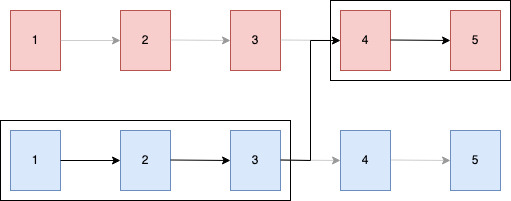
\includegraphics[width=6.5cm]{stitch.jpg}
      \caption*{This diagram gives us a simple view of a stitched network. The black arrows denote the flow of data, while
      the grey arrows denote the flow of data that would have been present, had the two networks been used without stitching.
      The different blocks denote different layers (numbered) and the different colors denote different neural networks. The arrow
      from layer 3 of the blue network to layer 4 of the red network involves a simple stitch transformation, though it is left
      out of the image for concision. The boxed layers, plus the stitch, make up the stitched network. In this specific case,
      the stitched network's task accuracy measures the similarity of red layer 3 with blue layer 3, since red layer 4 expects the
      input to come from red layer 3. However, we have no way of telling (given just the task accuracy) whether the representation
      from blue layer 3 to red layer 4 is the same as the representation from red layer 3 to red layer 4 or some other representation
      that yields similar results.}
   \end{figure}
\end{center}

\section*{Experimental Setup}
\subsection*{Models and Dataset}
We use the CIFAR-10 dataset\footnote{In the future, once our preliminary results are more interpretable, we intend to
continue on to imagenet.} with small ResNets. With our augmented class of stitches we compare all different
layers of ResNet18, ResNet34, and all
ResNets with between 10 and 18 layers. These small ResNets we characterize with four-tuples,
$R(x_1, x_2, x_3, x_4)$, where we choose $x_i \in \{1, 2\}$. For any of these ResNets there are, between an initial convolutional
layer and a final linear classification layer, four sets of Residual blocks numbered 1 through 4 and denoted by
$x_i$. Each set has either 1 or 2 blocks denoted by the value of $x_i$. Within each block there are two layers,
though we focus on stitching out of and into blocks, instead of the layers within them. 

Because within each block there are two layers, and there is one
additional initial convolutional layer as well as one additional classification layer, the total number
of layers is given by
\[2 + \sum_{i=1}^{i=4} 2 \cdot x_i \]

This means that for $R(1, 1, 1, 1)$ there are 10 layers, while for $R(2, 2, 2, 2)$ there are 18 layers. We call
$R(2, 2, 2, 2)$ by the shorthand, ``ResNet18'', though this should not be generalized because there are pairs
of networks with the same total number of layers but different numbers of blocks per tuple. For example:
$R(1, 1, 2, 2)$ and $R(2, 2, 1, 1)$ both have 14 layers. These ResNets are qualitatively different
because the blocks corresponding to each different set have different shapes. Specifically, the blocks in
the set corresponding to $x_1$ have depth 64, width 32, and height 32; the blocks corresponding to $x_2$ have
depth 128, width 16, and height 16; and in general the depth doubles each iteration,
while the height and width each halve.

It should be noted that ResNet34 is not a particularly special case. It is in fact $R(3, 4, 6, 3)$. In general,
a large class of high-accuracy ResNets, both small and large, can be produced by by picking different values for
$x_1, x_2, x_3, x_4$. We constrain $x_i$ to be either 1 or 2 since CIFAR-10 is a relatively easy task.

\subsection*{Experiment}
We train ResNet34 as well as each possible $R(x_1, x_2, x_3, x_4)$ as described above. There are $2^4 = 16$ such possible
small ResNets since each set of blocks can have either 1 or 2 blocks and there are 4 blocks. We stitch every unique ordered
pair of networks from this set. There are $16 \cdot 16$ such unique ordered pairs, yielding 256 total pairs to stitch.
For every pair we stitch every layer from the first network into every layer for the second. Note that we also stitch
every layer from ResNet18 to ResNet34 and vice versa as a special case of a ``medium-sized'' ResNet.

We use randomly initialized ResNets as controls. Unlike Bansal et al. we only vary our neural networks by their
initialization weights. For every pair of networks that are stitched, we also create a random sender and a random
reciever both with the same architecture as the sender and reciever respectively. Just as the sender is stitched
into the reciever, the random sender is stitched into both the reciever and the random reciever, and the sender
is also stitched into the random reciever. This allows us to acertain that the stitches
are not overly powerful [Bansal et al.].

We train each stitch for 4 iterations. This hyperparameter was selected after much experimentation. For both
regular training of the network and training of the stitches we use stochastic gradient descent with momentum 0.9,
batch size 256, weight decay 0.01, learning rate 0.01, and a post-warmup cosine learning rate scheduler.
 These hyperparameters were also arrived at from experimentation.

For each stitch, we plot the accuracy on a grid based on the sending layer and the reciever layer. The layer is
denoted by an integer which counts how many layers came before it.

As a bonus we also train a set of "similarity-trained" stitches. These stitches are also used as a sort of control and
their motivation explained more fully later. Most importantly, though, they are trained using mean squared error (and the
same hyperparameters) to copy the expected representation of the reciever using that from the sender.

\section*{Results}
\subsection*{Preliminary Results}
All our experimental results are formatted as layer to
layer similarity matrices. (The row is the sender, the column is the reciever, and the compared layers are the expected sender
and the sender; the entry is the accuracy of the stitched network).

Every single pair in our experiment has the same
patterns. When two random networks are stitched, all possible stitches have low accuracy with a rather uniform distribution. When
a sender is stiched with a random reciever, only stitches from the later layers of the sender into the later layers of the (random)
reciever have high stitching accuracy. When a random sender is stitched into a reciever, only stitches into the early layers of the
reciever have high stitching accuracy. When the sender is stitched into the reciever, all layers in the lower left hand triangle
of the layer-to-layer similarity matrix have high stitching accuracy. 
This intruiging last result was most apparent for small ResNets or different shapes.
Figures are below for all our results.

For larger ResNets of the same shape we saw more of a diagonal pattern (akin to Bansal et al.) though, the lower left hand triangle for small
resnets had higher
accuracy than the top right hand triangle by a lot. 
The cause for the triangle for smaller networks is mysterious. We believe that
it is possible that the stitch is not learning to emulate the expected representation but instead create another representation
that yields the same results (i.e. high accuracy). We are using a rough numerical estimate to understand this. Namely, we
are using the mean squared error between the expected representation and the representation produced by the stitched network.
We provide statistics and an analysis below. We also provide the results of a similarity-trained set of stitches which
try to copy the expected representation. These are meant mainly to give us a sense of how close a stitch could be to the
expected representation if it were "trying" to copy it. We find that these similarity-trained stitches are not very good
and perhaps not that similar from the corresponding normal (sometimes called "vanilla") stitch.

\begin{center}
   \begin{figure}[h!]
      \centering
      \caption{Triangle Pattern in Small ResNets}
      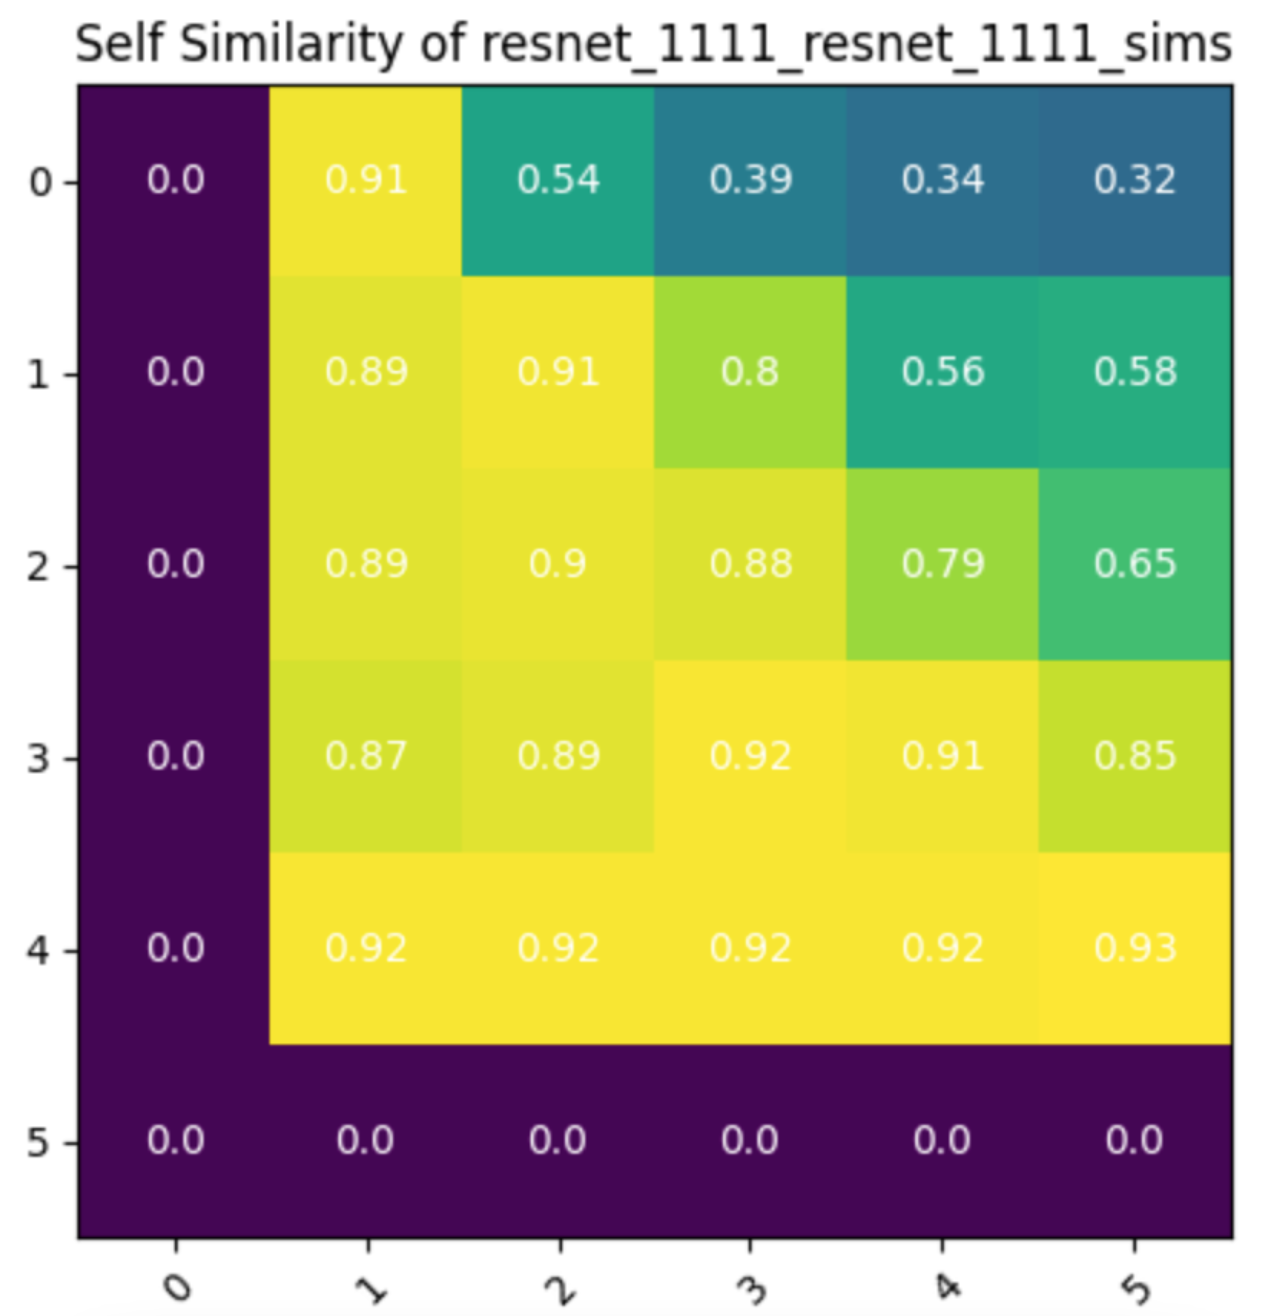
\includegraphics[width=6.5cm]{resnet1111_1111.png}
      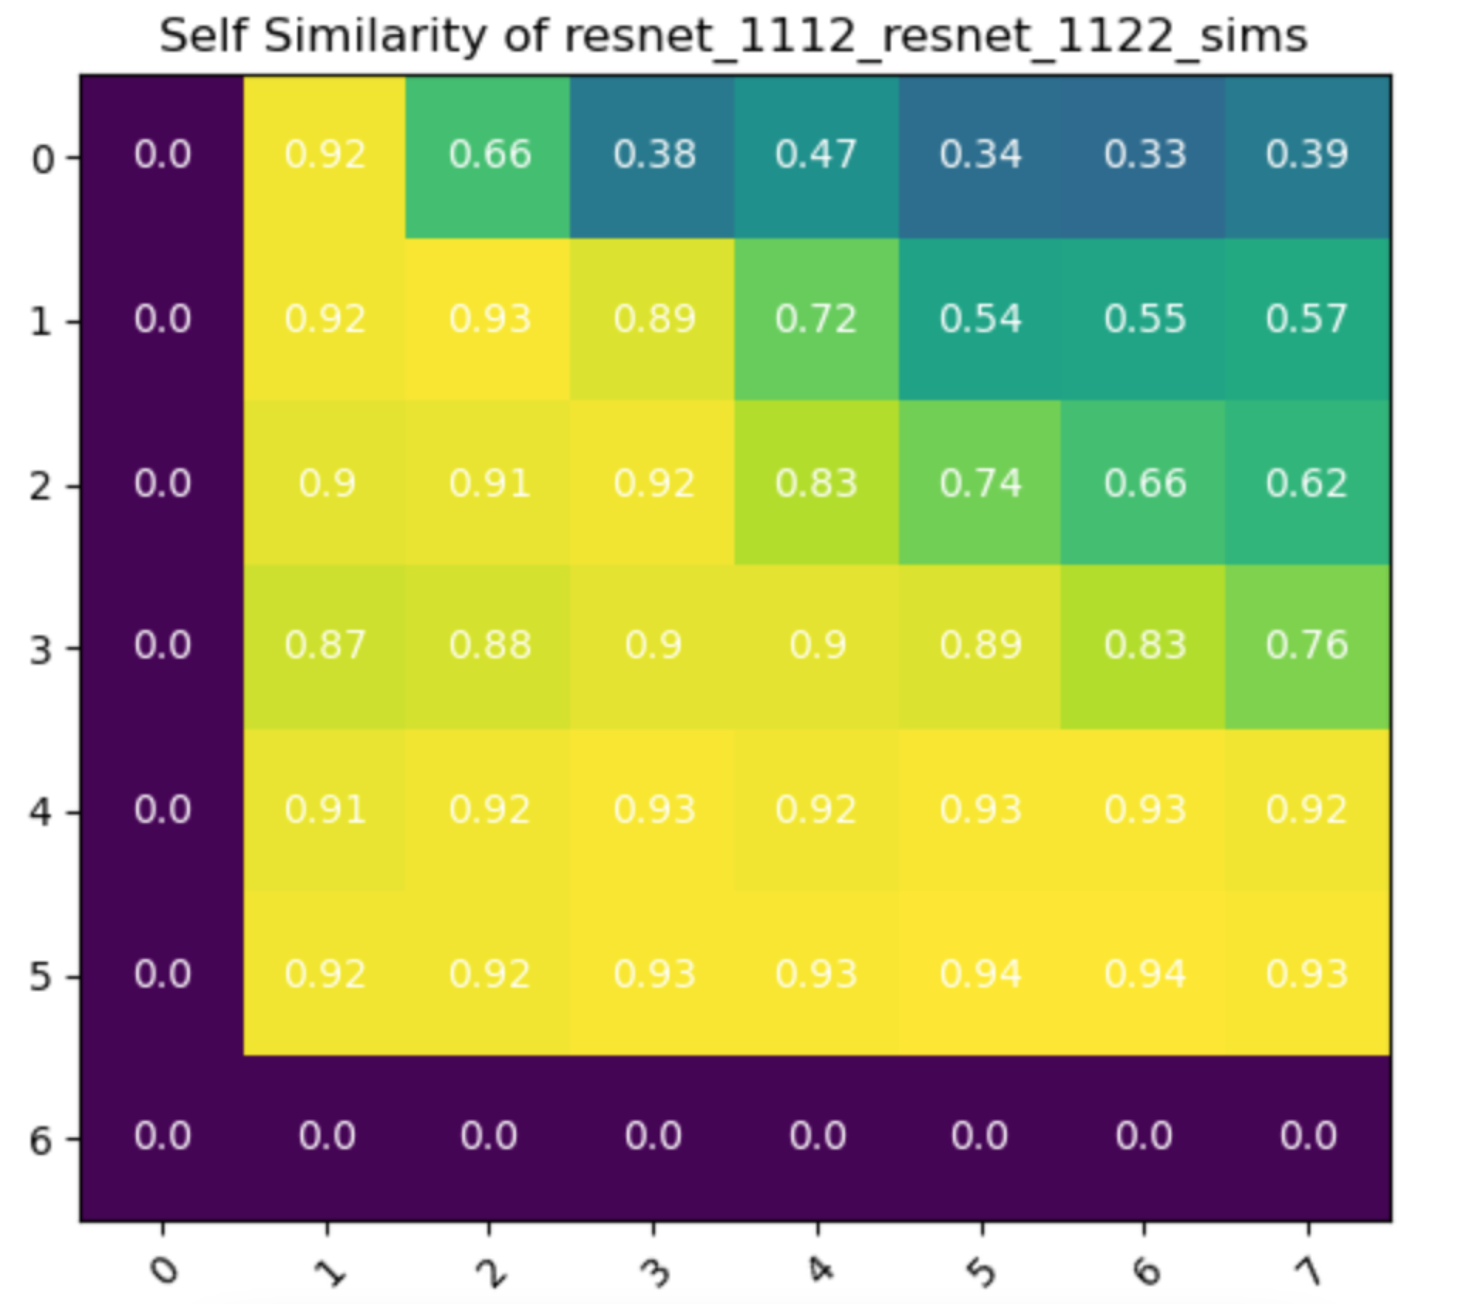
\includegraphics[width=6.5cm]{resnet1112_1122.png}
      \caption*{These are similarity matrices from sender to reciever. The row tells you the sending layer and the column tells you the recieving layer.
      The entry tells you the accuracy of the stitched model created by stitching between those two layers.}
   \end{figure}
\end{center}

\begin{center}
   \begin{figure}[h!]
      \centering
      \caption{Sometimes a Diagonal in Large ResNets}
      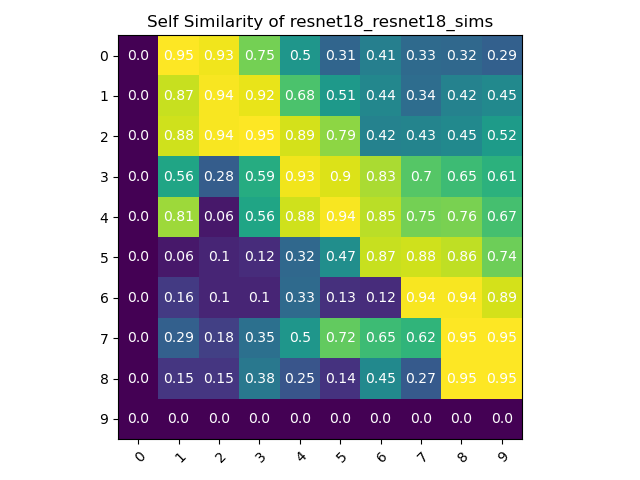
\includegraphics[width=8.5cm]{resnet18_resnet18_sims.png}
      \caption*{Similariy matrix from sender to reciever.}
   \end{figure}
\end{center}

\begin{center}
   \begin{figure}[h!]
      \centering
      \caption{Sometimes Triangular Pattern in Large ResNets}
      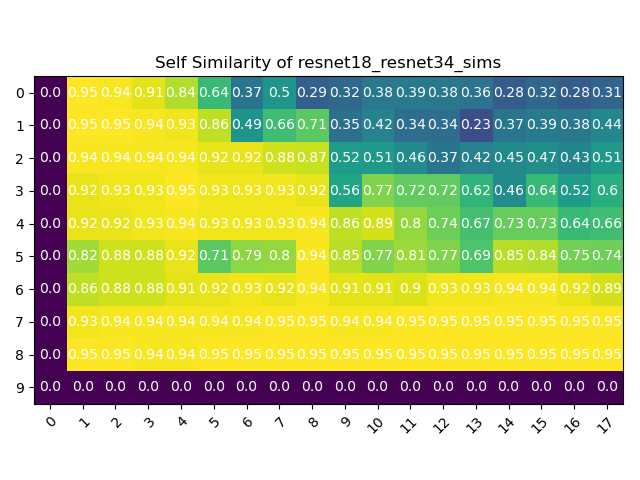
\includegraphics[width=9.5cm]{resnet18_resnet34_sims.png}
      \caption*{Similariy matrix from sender to reciever.}
   \end{figure}
\end{center}

\subsection*{Controls}
As previously mentioned we used random networks to control for stitching power. Nothing particularly interesting
came out of our controls. This was as we had hoped. A couple examples are below in figure 5. The main result from the controls
was that as the randomly initialized (untrained) fraction of the stitched network grew, the accuracy went down.

\begin{center}
   \begin{figure}[h!]
      \centering
      \caption{Triangle Pattern in Small ResNets}
      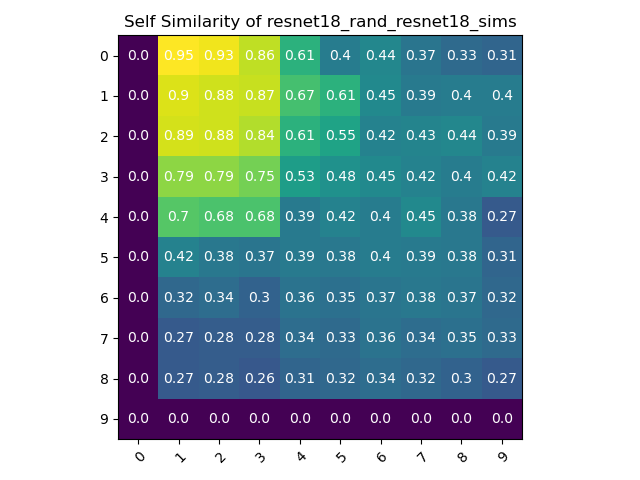
\includegraphics[width=8.5cm]{resnet18_rand_resnet18_sims.png}
      \caption*{These are similarity matrices. The row tells you the sending layer and the column tells you the recieving layer.
      The entry tells you the accuracy of the stitched model created by stitching between those two layers.}
   \end{figure}
\end{center}

\subsection*{Interpretation}
\subsubsection*{What We Had Expected}
The reason that these results are perplexing is that we were expecting to see some sort of diagonal in the similarity matrix
when stitching
different networks. Bansal et al.'s findings suggested that there would be a one-to-one layer correspondence between
two networks of the same architecture. While we did, roughly, see this for ResNet18 and ResNet34, we did not for the
small ResNets. Obviously, it is impossible to have a diagonal when the sender and reciever have different lengths,
but we had considered a few possibilities.

Namely, we considered that there may be a one-to-one correspondence between subsections of each neural network to
form some kind of ``strided diagonal''. In the layer one-to-one correspondence case, we interpret the correspondence
to tell us that the layers are learning the same representation. In the subsection one-to-one correspondence case
(the ``strided diagonal'') we interpret that to mean that there are black-box sections of each neural network which
have the same final learned representation.

To make our language more precise we can define consecutive sequences of neural networks as ``modules''. Naturally,
modules have modules within them and, if they are not the entirety of the network, they are within a module. We thought
that there would be some non-trivial modular mapping between two networks. That is to say, there would be some way of
describing the sender as a sequence of modules and the reciever as a sequence of modules, such that a mapping existed
between the two sequences. Obviously, the trivial mapping exists between the entire sender to the entire reciever
(since they both input identical images and both output nearly identical classifications), but we had hoped for more.

Implicit in our expectations, naturally, was the assumption that there would be a \textbf{mapping} between some quantity
in the sender and some other quantity in the reciever. It is highly unintuitive that layers in the sender are equally
similar (and very much so) to lots of layers in the reciever. We expected each layer to have at most one to three layers
in the other network it was similar to. As we've seen, however, later layers tend to be similar to nearly all earlier layers
by our stitching metric.

\subsection*{What This Might Mean}
We see two main explanations for the results: small ResNets on CIFAR-10 could be able to maintain most if not all of the image
information throughout their processing of the image and the stitches are learning to create representations which yield high
accuracy despite being different from their expected counterparts.

The former option is very interesting because it upheaves our understanding of neural networks. Normally we assume that
as data is more deeply processed in neural networks it becomes more ``high level'' and granular information is lost. If
this were not the case it would prompt us to understand when and why that is so. The latter option is compelling mainly
because it helps us find a limitation of stitching. In a sense it would mean that stitches are powerful enough to ``hack''
the reciever network: to trick it into using a representation it was not expecting. If this were possible and common, then
high stitching accuracy would not be a sign of similarity, though low stitching accuracy could be a sign of dissimilarity.

We mainly examine the latter option by using a similarity-trained stitch and by taking statistics on the mean squared
error (difference) of the stitches with respect to (mainly) the expected representation. A high mean squared error would
imply that the stitch is more likely to be different, while a low mean squared error would imply that the stitch is more
likely to be similar. It is a crude measurement, but we include it as a taste of what may be possible in the future. The
similariy trained stitch, on the other hand, is meant to give us a sense of how close a stitch could be to the expected
representation if that were it's only ``goal''. In both cases we use controls in the form of stitches with or between
random networks.

\subsection*{Self-Similarity-Trained Stitch}
Below we have a heatmap of the task accuracy for the similarity-trained stitch. We found that it was not
easy to train a stitch exclusively using mean squared error with respect to the expected representation. We suspect
that there may be subspaces of the representation space that are far more relevant to accuracy and that by using
mean squared error the similarity-trained stitch has to try much, much harder to get any results (which it fails
to get here). For context, we only needed around 1 epoch to train regular, vanilla stitches to reach competitive accuracy
with the original network and around 4 to reach nearly identical accuracy. For the similarity-trained stitch, we used 30
epochs per stitch and have close to random accuracy.

\begin{center}
   \begin{figure}[h!]
      \centering
      \caption{Naive Self-Similarity Training Tends To Fail}
      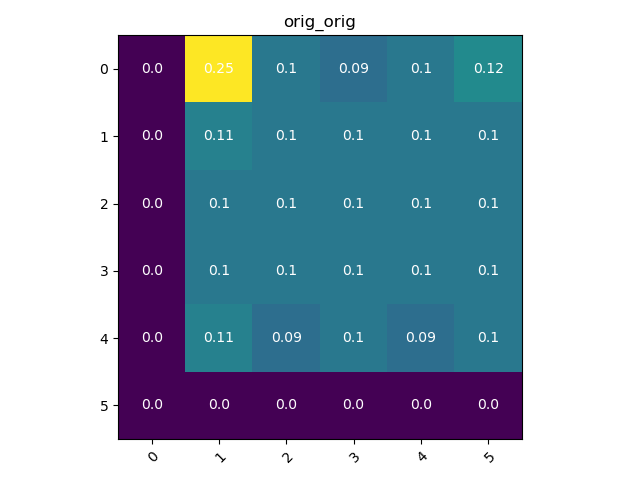
\includegraphics[width=7.5cm]{resnet1111_1111_autoencoder.png}
      \caption*{Similarity matrix from sender to reciever.}
   \end{figure}
\end{center}

\subsection*{Numerical Analysis}
We examined the diagonal of nine pairs of stitched networks: 2211 with 2211, 1211 with 1211, 
2121 with 2121, 2111 with 2111, 2221 with 2221, 1121 with 1121, 1112 with 1112, 1111 with 1111, 
and 1221 with 1221. We compared trained networks with random ones (and vice versa) as well as trained
networks with the same trained network and random networks amongst eachother.\footnote{NANs were encountered for 
Traineed to Random for both the autoencoder and vanilla stitches when comparing with the original on the diagonal.
This probably means  that there were
very large numbers which means that some distances were too long to be computed meaning implying that
the representations were totally, randomly, differnet. When we compared the entire tables, we got NANs and infinities
for various cases with random representations.}

That is to say, we measured the mean squared distance (frobenius norm) of the stitched representations for the networks
for each of those pairs of networks, specifically for the representations that were at the same layer. This enabled us
to get a sense for whether the networks were learning the same representation or "hacking" eachother.

We also computed the same statistics on the set of all stitches to see if the diagonal was any different. We focused
on the diagonal because due to Bansal et. al. we have more confidence in it corresponding to a true emulation of the
expected representation.

What we tended to find was that for random networks the mean squared distance was high and for trained networks it was
low. It tended to be around two orders of magnitude lower for the similarity-trained stitch, which is expected, but the
similarity trained stitch does not seem to be further from the expected representation than the vanilla stitch is from it
(in ``Self-Similarity Stitches vs. Vanilla Stitches''). The specifics (tables) are in the appendix.
   
\section*{Conclusion}
It appears that stitching does not behave for different architectures exactly as we had hoped, though it does not seem
to be generating representations altogether different from those that were expected. We hypothesize that in some cases
stitches may be able to ``hack'' the reciever by learning to give it novel representations which nonetheless yield high
accuracy. However, it appears that stitches do not deviate, numerically, that much from the expected representation on
average. Most likely, there are subspaces in the representation space more important than others and the vanilla stitch
is able to optimize them, potentially at the expense of others, thus yielding slightly higher mean squared error with
respect to the expected representation than is possible using a purely mean squared error trained stitch. We see this
by training such a stitch (the ``Self-Similarity'' stitch). In line with this conclusion, the similarity stitch struggles
to reach high accuracy, probably because it is to ``diversified'' and does not have information about what subspaces
matter more for the downstream task.

\section*{Appendix}
\subsection*{Diagonals: Vanilla Stitches}
\begin{tabular}{c c c c c}
   Name&Minimum&Mean&Maximum&Standard Deviation\\
   Trained to Trained&2.03e-03&4.41e-02&2.80e-01&6.10e-02\\
   Trained to Random&1.27e-01&4.28e+05&4.24e+06&1.12e+06\\
   Random to Trained&1.50e-02&3.25e-01&5.29e-01&1.56e-01\\
   Random to Random&1.58e-01&1.26e+02&1.36e+03&2.92e+02\\
\end{tabular}
\subsection*{Diagonals: Self-Similarity Stitches}
\begin{tabular}{c c c c c}
   Name&Minimum&Mean&Maximum&Standard Deviation\\
   Trained to Trained&2.15e-05&1.50e-02&1.91e-01&3.73e-02\\
   Trained to Random&5.52e-02&7.60e+04&3.56e+05&1.26e+05\\
   Random to Trained&3.48e-05&1.10e-03&5.91e-03&2.01e-03\\
   Random to Random&1.73e-02&4.94e+00&6.03e+01&1.27e+01\\
\end{tabular}
\subsection*{Diagonals: Self-Similarity Stitches vs. Vanilla Stitches}
\begin{tabular}{c c c c c}
   Name&Minimum&Mean&Maximum&Standard Deviation\\
   Trained to Trained&1.21e-03&2.33e-02&1.14e-01&3.89e-02\\
   Trained to Random&2.71e-03&1.67e+05&3.67e+06&7.32e+05\\
   Random to Trained&7.94e-03&3.23e-01&5.29e-01&1.59e-01\\
   Random to Random&1.17e-01&1.18e+02&1.35e+03&2.86e+02\\
\end{tabular}
\subsection*{All Representation Pairs: Vanilla Stitches}
\begin{tabular}{c c c c c}
   Name&Minimum&Mean&Maximum&Standard Deviation\\
   Trained to Trained&1.63e-03&4.49e-02&3.63e+00&1.37e-01\\
   Trained to Random&1.55e-04&2.63e+05&1.78e+07&1.00e+06\\
   Random to Trained&1.35e-02&2.21e+00&2.27e+02&1.17e+01\\
   Random to Random&1.34e-01&7.25e+04&1.24e+07&5.94e+05\\
\end{tabular}
\subsection*{All Representation Pairs: Self-Similarity Stitches}
\begin{tabular}{c c c c c}
   Name&Minimum&Mean&Maximum&Standard Deviation\\
   Trained to Trained&5.39e-06&1.58e-02&1.32e+00&5.90e-02\\
   Trained to Random&1.71e-07&1.06e+05&9.19e+06&4.27e+05\\
   Random to Trained&6.32e-06&2.05e-03&1.88e-02&4.31e-03\\
   Random to Random&1.59e-02&4.20e+04&6.90e+06&3.44e+05\\
\end{tabular}
\subsection*{All Representation Pairs: Self-Similarity Stitches vs. Vanilla Stitches}
\begin{tabular}{c c c c c}
   Name&Minimum&Mean&Maximum&Standard Deviation\\
   Trained to Trained&7.83e-04&1.98e-02&5.87e-01&3.25e-02\\
   Trained to Random&1.54e-04&6.26e+04&5.79e+06&3.43e+05\\
   Random to Trained&7.94e-03&2.21e+00&2.27e+02&1.17e+01\\
   Random to Random&9.44e-02&2.12e+04&4.77e+06&2.08e+05\\
\end{tabular}

% \section{Experimental Setup}
% % Notational notes for myself:
% %    %% Stitching %%
% % A_{i,j} is the module from i to j inclusive
% % A_{\leq N} is the prefix (i.e. module from 0 to N inclusive)
% % A_{\geq K} is the suffix of all layers after K.
% % AB_{i \rightsquigarrow | \rightarrow \not{\rightarrow} j} is the stitch from A to B from layer i to layer j
% %   depeneding on whether the accuracy is unknown, high, or low (so representations are unknown, similar, or differnet)
% % To refer to the outputs of networks we use the letter R for representation. For the output of network A
% % from layer i we use R_{A, i}. This'd be the input for network A at layer i + 1 or some sort of stitch.
% %    %% Mappings %%
% % A \rightarrow B
% % 
% % 
% \subsection{Definitions}
% We begin with a lot of definitions and then proceed to elucidate the high-level experimental setup
% and preliminary results. Our goal from the experiments is to understand what functionality is shared
% across pairs of neural network architectures. We rely heavily on a domain-specific language defined
% below because it allows us to ascribe terms with precise meaning to all the different types of behaviors
% we expect to see.

% \subsubsection*{Basic Definitions and Terminology}
% \begin{itemize}
%    \item Representation: the intermediate output of a neural network, usually refered to as \(R_{A, i}\) if output from layer \(i\) of network \(A\).
%    \item Prefix: the first \(N\) layers of a neural network, \(A\). We may call the prefix function \(A_{\leq N}\) or \(A_{<N+1}\) if applicable.
%    \item Suffix: the last layers of a neural network \(B\), starting at layer \(K\). We may call the suffix function \(B_{\geq K}\) or \(B_{>K-1}\) if applicable.
%    \item Module: a subsequence of consecutive layers in a neural network, similar to the notion of a substring in computer systems. It can also be thought of as a prefix of a suffix, or a suffix of a prefix. It is denoted with the start and ending layers (inclusive). For example \(C_{2,3}\) is the module with layers 2 and 3 of network \(C\). During normal computation, the first layer outputs into it, and it outputs into the fourth layer. Note that single layers are also modules. \(C_{1,1}\) is both the first layer and the first possible module of \(C\). Moreover, prefixes and suffixes are modules.
%    \item Submodule: a module inside a module. for example, \(C_{2,2}\) is a submodule of \(C_{2,3}\). This will be used when we wish to describe the internals of modules.
%    \item Supermodule: a module within which there is a module. This will be used when we wish to group modules.
%    \item Sender: when a module recieves input from a previous module we call that previous module the sender. We may also say that a module is \emph{sending} when we wish to express that it is the sender.
%    \item Reciever: The module some other module is sending to. We may also say that it is \emph{recieving}.
%    \item Expected sender (or reciever): absent of stitching, the module that would be the sender or the reciever to/from the current module.
%    \item Expected input (or output): the output of the expected sender or reciever during normal computation.
% \end{itemize}

% \subsubsection*{Stitching}
% We define stitching in the same way as Bansal et. al. 
% Say we wish to stitch two networks \(A\) and \(B\).
% We will calculate the output of a prefix of \(A\),
% input it into our stitch \(S\), and then input the output
% of \(S\) into a suffix of \(B\). Say we take the
% output of \(A\) at layer \(i\), input it into \(S\),
% and then take the output of \(S\) and input it into
% \(B\) at layer \(j+1\). We say that layer \(i\) of
% \(A\) was stitched \emph{into} layer \(j+1\) of \(B\).
% The composition \(S \circ A_{\leq i}\) has replaced
% the expected sender, \(B_{\leq j}\) of \(B_{>j}\).
% As discussed by Bansal et. al, this enables us to compare
% the representations \(R_{A,i}\) and \(R_{B,j}\).

% The stitch \(S\) is a function whose domain is the set of possible \(R_{A,i}\)
% and whose range is in the same space as \(R_{B,j}\). For the same reasons as Bansal et. al.
% we use simple function classes like 1x1 convolutions where applicable and strided convolutions
% elsewhere.

% The network formed with \(B_{\geq j+1} \circ S \circ A_{\leq i}\) is called the 
% \emph{stitched network} and is often denoted as \(AB_{i \rightsquigarrow j+1}\). The stitched 
% network is frozen in all layers except for \(S\), which is trained with gradient descent
% so as to approximate the best possible choice for \(S\). If the resulting accuracy
% is high then we refer to the stitched network as \(AB_{i \rightarrow j+1}\) and we say
% that \(A\) is \emph{stitchable} to \(B\) through those layers: \(\exists AB_{i \rightarrow j+1}\).
% If the resulting accuracy is low, we refer to the stitched network as \(AB_{i \not{\rightarrow} j+1}\)
% and we say that \(A\) is not stitchable to \(B\) through those layers.

% \subsubsection*{Representational Mappings}
% A representational mapping between neural networks \(A\) of length and \(B\) is a mapping that assigns
% at most one \(R_{B,j}\) for every \(R_{A,i}\). We sometimes use the layer indices \(i\) and \(j\)
% as shorthand.

% We establish the mapping as follows: for each valid \(i\) in \(A\), find the \(j\) in \(B\)
% such that \(R_{A,i}\) is most similar to \(R_{B,j}\) out of all possible \(j\) and
% \(\exists AB_{i \rightarrow j+1}\). We refer to the mapping as \(A \rightarrow B\). There are
% other ways to define such a relation, but we pick this one for simplicity.
% Intuitively this says that those two representations are, to an extent, interchangeable.
% We also hope that this mapping will be injective and monotonic.
% By monotonic we simply mean that if \(i_{1} < i_{2}\), \(i_{1}\) maps to \(j_{1}\),
% and \(i_{2}\) maps to \(j_{2}\), then it should be the case that \(j_{1} < j_{2}\). This simply
% means that the network is learning more abstract notions as data flows through it.

% The precise reader will note that while the representations may be interchangeable in one direction
% they may not be in both, depending on the type of stitch. That is to say,  \(\exists AB_{i \rightarrow j+1}\)
% does not imply \(\exists BA_{j \rightarrow i+1}\), even with linear transformations and 1x1 convolutions
% because of the possibility of drastic changes in dimensionality. We use \(\rightarrow\) and \(\leftarrow\)
% or flip the order of the operands to differentiate the two directions.
% When we wish to express \(\exists AB_{i \rightarrow j+1} \land \exists BA_{j \rightarrow i+1}\),
% we may often say \(AB_{i \leftrightarrow j}\). We may also define a two-way representational mapping,
% \(A \leftrightarrow B = (A \rightarrow B) \cap (B \rightarrow A)\), though it is not a mapping
% in the mathematical sense, but instead a list of tuples.
% % Begin Footnote
% \footnote{For a set of tuples \(C\), Define the reverse tuple set \(V(C) = \{(b, a) \forall (a, b) \in C\}\).
% For a mapping \(f: D \to R\) we define its set of tuples, \(T(f) = \{(x, f(x)) \forall x \in D\}\).
% For \(f: D \to R, g: R \to D\), we define \(f \cap g = T(f) \cap V(T(g))\). We can also define
% \(f \cup g = T(f) \cup V(T(g))\). Note that \(f \cap g\) is always a subset of \(D x R\), and
% that \(f \cap g = V(g \cap f)\)}.
% % End Footnote

% The precise reader will also note that high accuracy should be relative to some baseline. We define what is high
% experimentally and using random (untrained) networks. When stitching different architectures we compare the accuracy
% with that of the \emph{least accurate} architecture that went into the stitch. That means that if we stitch from
% a very large (or wide) network to a very small one, or vice versa, we should expect the smaller network to be a
% bottleneck on accuracy.

% \subsubsection*{Modular Mapping}
% Using our representational mappings, we establish a more general notion of modular mappings based on modules. A Modular mapping
% tells us about what modules in two different neural networks might have shared functionality based on representational similarity.
% Intuitively, if one module is mapped to another, then the latter can be swapped out for the former, with two stitches, in the latter's network.
% Informally, for two networks \(A\) and \(B\), \(A_{i_1, i_2}\) is mapped to \(B_{j_1, j_2}\) if we can find a pair of stitches \(S_1, S_2\), such that the accuracy is high for
% \(B_{>j_2} \circ S_2 \circ A_{i_1,i_2} \circ S_1 \circ B_{<j_1}\). Since it's possible to infer this from \(A \rightarrow B\) and \(B \rightarrow A\),
% however, we infer it from \(\exists BA_{j_1 \rightarrow i_1}\) and \(\exists AB_{i_2 \rightarrow j_2+1}\).

% To find these modular mappings we can simply brute force for all possible indices, \(i_1, i_2, j_1, j_2\),
% given our pre-computed representational mappings. If we denote the length (in layers) of \(A\) as \(N_1\) and
% that of \(B\) as \(N_2\), The runtime of the brute force algorithm is \(\mathcal{O}(\alpha N_1 N_2)\) where \(\alpha\) is
% the worst-case time necessary to optimize a stitch between any pair of layers.

% However, we would prefer to also try and enforce monotonicity of the modular mapping. If two modules, \(M_1 = A_{i_1, i_2}, M_2 = A_{i_3, i_4}\),
% have the property that \(i_2 < i_3\), we say that \(M_1 < M_2\). Monotonicity means that of we have any two modules in \(A\),
% \(M_{A_1}, M_{A_2}\), and any two modules in \(B\), \(M_{B_1}, M_{B_2}\), such that \(M_{A_1} \Rightarrow M_{B_1}\)
% and \(M_{A_2} \Rightarrow M_{B_2}\), then \(M_{A_1} < M_{A_2}\)implies \(M_{B_1} < M_{B_2}\). Monotonicity is preferable, because
% it makes the mapping more interpretable. It may not be the case that the modular mapping is monotonic, but we can instead choose to
% focus on a subset of module pairs that is. We present an algorithm below which given two neural networks finds a monotonic subset of
% \(A \Rightarrow B\).

% \begin{center}
% \begin{algorithm}
% \caption{Find A Monotonic Modular Mapping Subset}
% \begin{algorithmic}[h]
% \Procedure{MFind(\(A\), \(B\))}{}
%       \State Pretrain and Freeze \(A\) and \(B\) seperately
%       \State \(A\) has length \(N\)
%       \State \(B\) has length \(M\)
%       \State Find \(A\rightarrow B\) through brute force
%       \State Find \(B\rightarrow A\) through brute force
%       \State \(i_{start} = 1\)
%       \State \(j_{start} = 1\)
%       \State Initialize \(MM = \{\}\)
%       \For{\(i_{end} \in [1, N-1]\)}
%          \For{\(j_{end} \in [j_{start}, M-1]\)}
%             \If{\((B_{j_{start}-1} \rightarrow A_{i_{start}}) \land (A_{i_{end}} \rightarrow B_{j_{end}+1})\)}
%                \State Add \((A_{i_{start}, i_{end}}, B_{j_{start}, j_{end}})\) to \(MM\)
%                \State \(i_{start} = i_{end} + 1\)
%                \State \(j_{start} = j_{end} + 1\)
%                \State Break Inner Loop
%             \EndIf
%          \EndFor
%       \EndFor
%       \State Return \(MM\)
% \EndProcedure
% \end{algorithmic}
% \end{algorithm}
% \end{center}

% \subsection{Hypotheses}
% Now that we know how to talk about modules, we introduce 4 main idealized cases that may present themselves when we
% try to modularly map two different neural networks of different sizes. We assume that these mappings are all monotonic.
% We describe these assuming that the sender network is at most as long as the reciever network.

% \begin{itemize}
%    \item Layer to layer (L2L) mapping: single layers (in shorter networks) may have the same functionality as single layers in longer networks. Additional layers in longer networks introduce new functionality. This mapping is injective, but not necessarily surjective.
%    \item Layer to module (L2M) mapping: single layers (in shorter networks) may have the same functionality as modules in longer networks. The long networks have the same functionality, but better. This mapping is injective and ideally surjective.
%    \item Module to module (M2M) mapping: modules (in shorter networks) may have the same functionality as modules in longer networks. This mapping is injective and ideally surjective.
%    \item No (N) mapping: informally, when there is M2M mapping, but the modules are so big as to be uninformative.
% \end{itemize}

% It is possible that our mappings will not be monotonic, but we hope to find that they are. It is an elegant
% simplifiying assumption.

% Given this assumption, it is (only) possible to have these four cases outlined above. However, which one
% is most prevalent at a specific segment of a network may change: we may start with L2L mappings followed by
% M2M or N mappings, for example. To define a notion of this, we introduce \textit{realms}. Realms are pairs
% of supermodules within which submodules obey a single mapping mode (L2L, L2M, M2M, or N).
% More generally, if within a pair of supermodules behavior follows some pattern, we label it a realm.

% Thus, we may re-pharse our goal as that of describing the realms of modular mappings for different
% neural network architectures. To do this we generate a monotonic modular mapping based on representational
% mappings which we found using stitching. This helps us understand for pairs of networks, where they have the
% same functionality in a precise way.

% \subsection{Networks and Dataset}
% We focused on varying only the random seed of the neural network. To simplify our analysis we also used the CIFAR-10 dataset
% with standard resnets. These currently only include ResNet18, but will soon also include  ResNet34, ResNet50, ResNet101, ResNet152.
% The optimizers and hyperparameters used are further elucidated in the appendix.

% For layers with the same width and height we used 1x1 convolutions as our stitching function class. For layers with different dimensions
% we utilized the fact that the dimensions of the layers are powers of two (in our networks). In stitches that required downsampling (due
% to smaller dimensions in the reciever) we used strided convolutions. In stitches that required upsampling we simply used a nearest
% upsampling followed by a 1x1 convolution (which you can think of as reversed strided convolutions).

% \subsection{Tests and Controls}
% \subsubsection*{Networks of the same architecture}
% First we stitched networks of each architecture with other networks of the same architecture. We trained lists of networks for each 
% architecture. For each list we called the first element the \textit{pivot}. The pivot was stitched to each of the other networks
% in the same list, including itself. For every pair of networks we stitched each layer in the sender network to each layer in the
% reciever network. 

% For the purpose of creating a control, we made sure that there was a random (untrained) reciever network in the list. We also swapped 
% pivots with another untrained network which was stitched with all the other networks in the list. This ensured that we had baselines
% for resulting accuracy (and therefore similarity).

% You can think of the result of each pair of networks' stitches as a square matrix of accuracies, where the row denotes the layer of the
% sender network and the column denotes the layer of the reciever network. The accuracy at that elements is our measure of representational
% similarity. These tables are tiled into a tensor which represents the results of the stitch. In the depth dimension we average to find
% the average similarity over all our experiments for that architecture. Note that we insert zero at layer pairs that are not stichable
% due to dissimilar shapes.

% \subsubsection*{Networks of different architectures}
% We will conduct the same experiment as above, but where the pivot (sender) architecture is different from the reciever architecture.
% For each pair of architectures, we pick a pivot of each architecture along with a (small) list of recievers of the other architecture.
% We then repeated the procedure from the case with two identical architectures. Note that instead of a square matrix of accuracies, we
% have a rectangular matrix of accuracies. This matrix will be tall if the sender network is longer than the reciever network, and wide
% in the other case.

% \subsection{Testing Algorithm}
% More details will be elucidated in the appendix.

% \section{Results}
% \subsection{Summary}
% We have preliminary results that suggest the expected: networks of the same architecture yield a high similarity
% along the layer-to-layer matrix diagonal, with decreasing accuracies towards the top right and bottom left corners. This tells us
% that they are in a L2L realm (where corresponding layers have similar output representations and therefore functionality).
% For a random network, we have random behavior. We trained on a ResNet18 and have graphics below.
% \begin{center}
%    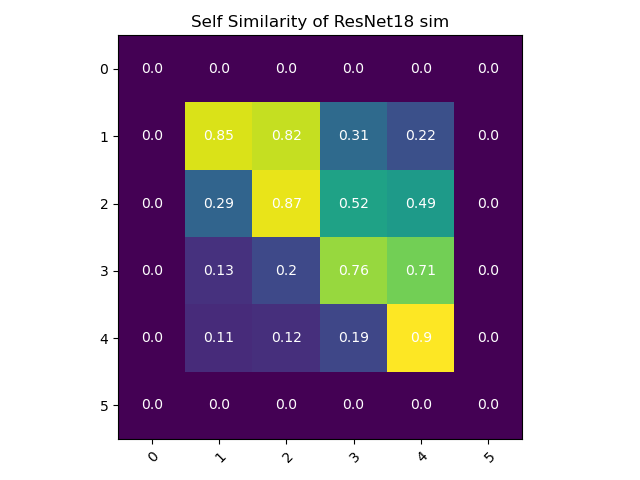
\includegraphics[width=6.5cm]{sim.png}
%    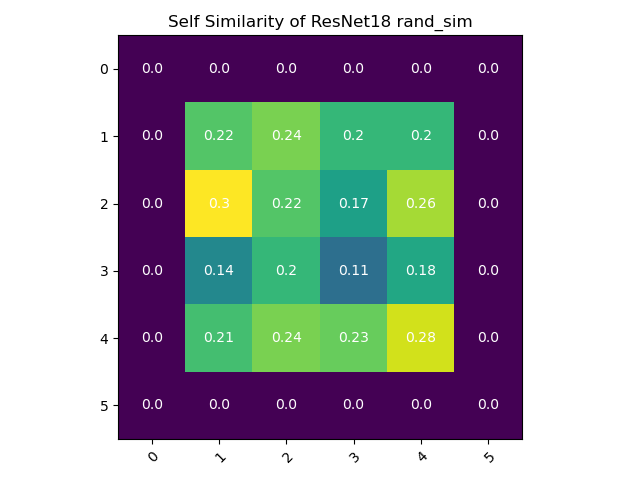
\includegraphics[width=6.5cm]{rand.png}
% \end{center}
% \subsection{Figures}
% ...

% % Figures that make sense when they are in black and white are ideal
% % \begin{figure}[h]
% % \begin{center}
% % %\framebox[4.0in]{$\;$}
% % \fbox{\rule[-.5cm]{0cm}{4cm} \rule[-.5cm]{4cm}{0cm}}
% % \end{center}
% % \caption{Sample figure caption.}
% % \end{figure}

% \subsection{Tables}
% ...

% % \begin{table}[h]
% % \caption{Sample table title}
% % \label{sample-table}
% % \begin{center}
% % \begin{tabular}{ll}
% % \multicolumn{1}{c}{\bf PART}  &\multicolumn{1}{c}{\bf DESCRIPTION}
% % \\ \hline \\
% % Dendrite         &Input terminal \\
% % Axon             &Output terminal \\
% % Soma             &Cell body (contains cell nucleus) \\
% % \end{tabular}
% % \end{center}
% % \end{table}

% \section{Analysis and Interpretation of Results}
% \subsection{Interpretation}
% ...
% % It didn't work.

% \subsection{Significance}
% ...
% % What this means for the future and the field.

% \section{Conclusions}
% ...
% % We'll write our conclusions in a nice format here.

% \section*{Acknowledgments}
% Thank you to the SuperUROP benefactors (MIT EECS) for funding this project.

% \bibliography{iclr2021_conference}
% \bibliographystyle{iclr2021_conference}

% \appendix
% \section{Appendix}
% ...

\end{document}
